% Important: If latex complains about unicode characters,
% please use "\usepackage[utf8x]{inputenc}" in your preamble
% You can change the size of the picture by putting it into the construct:
% 1) \resizebox{10cm}{!}{"below picture"} to scale horizontally to 10 cm
% 2) \resizebox{!}{15cm}{"below picture"} to scale vertically to 15 cm
% 3) \resizebox{10cm}{15cm}{"below picture"} a combination of above two
% It is not recomended to use the scale option of the tikzpicture environment.
\scalebox{0.8}{
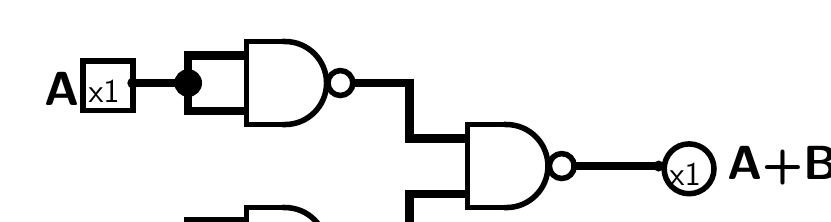
\begin{tikzpicture}[x=1pt,y=-1pt,line cap=rect]
\useasboundingbox (0,0) rectangle (280,60);
\def\logisimfontA#1{\fontfamily{cmr}{#1}} % Replaced by logisim, original font was "SansSerif"
\definecolor{custcol_0_0_0}{RGB}{0, 0, 0}
\definecolor{custcol_ff_ff_ff}{RGB}{255, 255, 255}
\draw [line width=3.0pt, custcol_0_0_0 ]  (198.0,50.0) -- (228.0,50.0) ;
\draw [line width=3.0pt, custcol_0_0_0 ]  (78.0,10.0) -- (58.0,10.0) -- (58.0,20.0) -- (58.0,30.0) -- (78.0,30.0) ;
\draw [line width=3.0pt, custcol_0_0_0 ]  (78.0,90.0) -- (58.0,90.0) -- (58.0,80.0) -- (58.0,70.0) -- (78.0,70.0) ;
\draw [line width=3.0pt, custcol_0_0_0 ]  (38.0,80.0) -- (58.0,80.0) ;
\draw [line width=3.0pt, custcol_0_0_0 ]  (38.0,20.0) -- (58.0,20.0) ;
\draw [line width=3.0pt, custcol_0_0_0 ]  (118.0,20.0) -- (138.0,20.0) -- (138.0,40.0) -- (158.0,40.0) ;
\draw [line width=3.0pt, custcol_0_0_0 ]  (158.0,60.0) -- (138.0,60.0) -- (138.0,80.0) -- (118.0,80.0) ;
\fill [line width=3.0pt, custcol_0_0_0]  (58.0,80.0) ellipse (5.0 and 5.0 );
\fill [line width=3.0pt, custcol_0_0_0]  (58.0,20.0) ellipse (5.0 and 5.0 );
\draw [line width=2.0pt, custcol_0_0_0]  (239.0,51.0) ellipse (9.0 and 9.0 );
\logisimfontA{\fontsize{12pt}{12pt}\sffamily\selectfont\node[inner sep=0, outer sep=0, custcol_0_0_0, anchor=base west] at  (232.0,57.0)  {x1};}
\fill [line width=2.0pt, custcol_0_0_0]  (228.0,50.0) ellipse (2.0 and 2.0 );
\draw [line width=2.0pt, custcol_0_0_0 ]  (20.0,72.0) -- (37.0,72.0) ;
\draw [line width=2.0pt, custcol_0_0_0 ]  (38.0,72.0) -- (38.0,89.0) ;
\draw [line width=2.0pt, custcol_0_0_0 ]  (38.0,90.0) -- (21.0,90.0) ;
\draw [line width=2.0pt, custcol_0_0_0 ]  (20.0,90.0) -- (20.0,73.0) ;
\logisimfontA{\fontsize{12pt}{12pt}\sffamily\selectfont\node[inner sep=0, outer sep=0, custcol_0_0_0, anchor=base west] at  (22.0,87.0)  {x1};}
\logisimfontA{\fontsize{16pt}{16pt}\fontseries{bx}\sffamily\selectfont\node[inner sep=0, outer sep=0, custcol_0_0_0, anchor=base west] at  (5.0,88.0)  {B};}
\fill [line width=2.0pt, custcol_0_0_0]  (38.0,80.0) ellipse (2.0 and 2.0 );
\draw [line width=2.0pt, custcol_0_0_0 ]  (20.0,12.0) -- (37.0,12.0) ;
\draw [line width=2.0pt, custcol_0_0_0 ]  (38.0,12.0) -- (38.0,29.0) ;
\draw [line width=2.0pt, custcol_0_0_0 ]  (38.0,30.0) -- (21.0,30.0) ;
\draw [line width=2.0pt, custcol_0_0_0 ]  (20.0,30.0) -- (20.0,13.0) ;
\logisimfontA{\fontsize{12pt}{12pt}\sffamily\selectfont\node[inner sep=0, outer sep=0, custcol_0_0_0, anchor=base west] at  (22.0,27.0)  {x1};}
\logisimfontA{\fontsize{16pt}{16pt}\fontseries{bx}\sffamily\selectfont\node[inner sep=0, outer sep=0, custcol_0_0_0, anchor=base west] at  (6.0,28.0)  {A};}
\fill [line width=2.0pt, custcol_0_0_0]  (38.0,20.0) ellipse (2.0 and 2.0 );
\draw [line width=2.0pt, custcol_0_0_0] (93.0,95.0) arc (90.0:-90.0:15.0 and 15.0 );
\draw [line width=2.0pt, custcol_0_0_0 ]  (93.0,65.0) -- (79.0,65.0) -- (79.0,95.0) -- (93.0,95.0) ;
\draw [line width=2.0pt, custcol_0_0_0]  (113.0,80.0) ellipse (4.5 and 4.5 );
\draw [line width=2.0pt, custcol_0_0_0] (93.0,35.0) arc (90.0:-90.0:15.0 and 15.0 );
\draw [line width=2.0pt, custcol_0_0_0 ]  (93.0,5.0) -- (79.0,5.0) -- (79.0,35.0) -- (93.0,35.0) ;
\draw [line width=2.0pt, custcol_0_0_0]  (113.0,20.0) ellipse (4.5 and 4.5 );
\draw [line width=2.0pt, custcol_0_0_0] (173.0,65.0) arc (90.0:-90.0:15.0 and 15.0 );
\draw [line width=2.0pt, custcol_0_0_0 ]  (173.0,35.0) -- (159.0,35.0) -- (159.0,65.0) -- (173.0,65.0) ;
\draw [line width=2.0pt, custcol_0_0_0]  (193.0,50.0) ellipse (4.5 and 4.5 );
\logisimfontA{\fontsize{16pt}{16pt}\fontseries{bx}\sffamily\selectfont\node[inner sep=0, outer sep=0, custcol_0_0_0, anchor=base west] at  (253.0,55.0)  {A+B};}
\end{tikzpicture}
}